\section{Deployment Diagram}

Il seguente deployment diagram rappresenta la distribuzione fisica dei componenti software dell'applicazione all'interno dei diversi nodi di esecuzione.\\
Il sistema è suddiviso in quattro nodi principali: \textit{device, server, database ed external system}. Ogni nodo contiene degli artefatti (file o pacchetti di codice che vengono deployati) e componenti di runtime.\\
Questi nodi interagiscono tra loro mediante opportuni protocolli di comunicazione.

\begin{figure}[H]
    \centering
    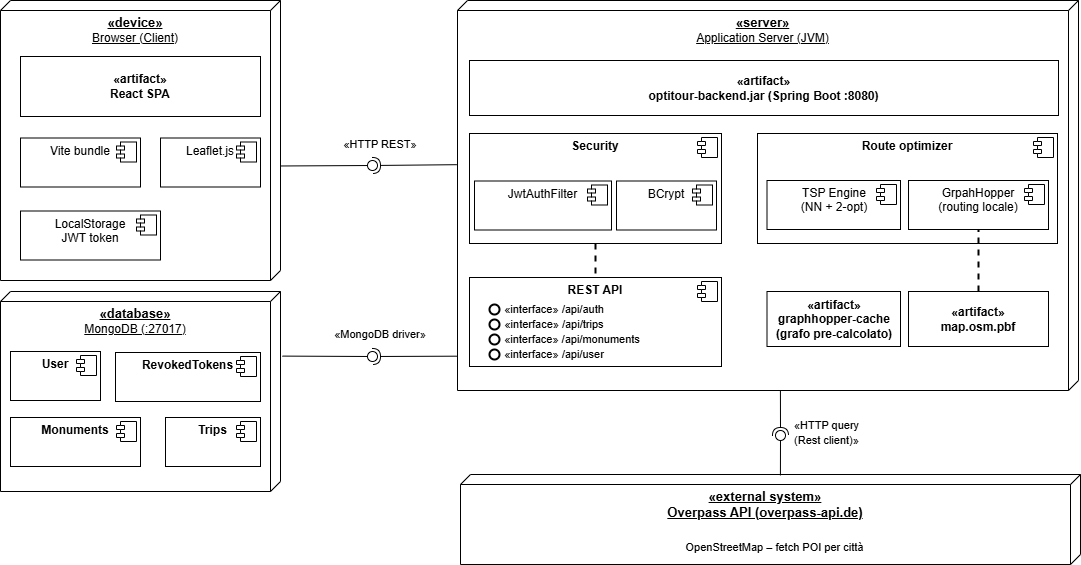
\includegraphics[width=0.75\linewidth]{Iterazione1/Diagrammi/DeploymentDiagram.png}
    \caption{Diagramma di deployment}
    \label{fig:DeploymentDiagram}
\end{figure}

\begin{itemize}
    \item \textbf{Nodo \guillemotleft device\guillemotright \ $\to$ Browser(client):} rappresenta il dispositivo dell'utente finale e contiene l'artefatto: \textbf{React SPA} che a sua volta è composto dal \textit{Vite bundle} e dalla libreria \textit{Leaflet.js} per la visualizzazione delle mappe.\\
    Il browser utilizza inoltre localStorage per memorizzare i JWT token necessari per l'autenticazione delle richieste verso il backend.\\
    La comunicazione verso il nodo server avviene tramite \textbf{HTTP REST } dove il token viene inserito nella header Authorization.
    
    \item \textbf{Nodo \guillemotleft server\guillemotright \ $\to$ Application Server(JVM):} rappresenta l'ambiente di esecuzione del backend basato su \textbf{Spring Boot} e distribuito come:\\
    \textbf{\guillemotleft artifact\guillemotright: optitour-backend.jar:} il quale viene esposto sulla porta :8080.\\
    All'interno del nodo sono presenti i seguenti componenti:
    \begin{itemize}
            \item \textbf{Sicurezza:} intercetta e valida le richieste mediante \textit{JwtAuthFilter} e si occupa dell'hashing delle password tramite \textit{BCrypt}.
            \item \textbf{REST API \ $\to$} esposte tramite gli endpoint: /api/auth, /api/trips,  /api/monuments e /api/user.
            \item \textbf{Motore di ottimizzazione:}
            \begin{itemize}
                \item TPS Engine (Nearest neighbor + 2-opt).
                \item GraphHopper per il routing locale.
            \end{itemize}
            \item  \textbf{Artefatti aggiuntivi}
            \begin{itemize}
                \item \textbf{\guillemotleft artifact\guillemotright map.osm.pbf:} dataset OpenStreetMap.
                \item \textbf{\guillemotleft artifact\guillemotright graphhopper-cache:} grafo pre-calcolato per il routing.
            \end{itemize}
            Il nodo server comunica con MongoDB tramite \textbf{Spring Data MongoDB} e con Overpass API tramite \textbf{HTTP query (REST client)}.
    \end{itemize}
    \item \textbf{Nodo \guillemotleft database\guillemotright \ $\to$ MongoDB:} rappresenta il database NOSQL utilizzato per la persistenza dei dati dell'applicazione.\\
    É esposto sulla porta :27017 e comunica con il backend tramite il driver MongoDB integrato in SpringData.
    \item \textbf{Nodo \guillemotleft eternal system \guillemotright \ $\to$ Overpass API:} rappresenta il sistema esterno basato su OpenStreetMap che viene utilizzato per il recupero dei POI (Point Of Interest) relativi ad una città.
    Il backend interagisce con esso mediante richieste \textbf{HTTP}, utilizzanto un client REST.

\end{itemize}

